\message{ !name(ISMIR2019template.tex)}% -----------------------------------------------
% Template for ISMIR Papers
% 2019 version, based on previous ISMIR templates

% Requirements :
% * 6+n page length maximum
% * 4MB maximum file size
% * Copyright note must appear in the bottom left corner of first page
% * Clearer statement about citing own work in anonymized submission
% (see conference website for additional details)
% -----------------------------------------------

\documentclass{article}
\usepackage[T1]{fontenc} % add special characters (e.g., umlaute)
\usepackage[utf8]{inputenc} % set utf-8 as default input encoding
\usepackage{ismir,amsmath,cite,url}
\usepackage{graphicx}
\usepackage{color}

% Optional: To use hyperref, uncomment the following.
% \usepackage[bookmarks=false,hidelinks]{hyperref}
% Mind the bookmarks=false option; bookmarks are incompatible with ismir.sty.

% Title.
% ------
\title{Using a parallel of Hausdorff dimension for pattern discovery in symbolic music data}

% Note: Please do NOT use \thanks or a \footnote in any of the author markup

% Single address
% To use with only one author or several with the same address
% ---------------
%\oneauthor
% {Names should be omitted for double-blind reviewing}
% {Affiliations should be omitted for double-blind reviewing}

% Two addresses
% --------------
%\twoauthors
%  {First author} {School \\ Department}
%  {Second author} {Company \\ Address}

%% To make customize author list in Creative Common license, uncomment and customize the next line
%  \def\authorname{First Author, Second Author}


% Three addresses
% --------------
\threeauthors
  {First Author} {Affiliation1 \\ {\tt author1@ismir.edu}}
  {Second Author} {\bf Retain these fake authors in\\\bf submission to preserve the formatting}
  {Third Author} {Affiliation3 \\ {\tt author3@ismir.edu}}

%% To make customize author list in Creative Common license, uncomment and customize the next line
%  \def\authorname{First Author, Second Author, Third Author}

% Four or more addresses
% OR alternative format for large number of co-authors
% ------------
%\multauthor
%{First author$^1$ \hspace{1cm} Second author$^1$ \hspace{1cm} Third author$^2$} { \bfseries{Fourth author$^3$ \hspace{1cm} Fifth author$^2$ \hspace{1cm} Sixth author$^1$}\\
%  $^1$ Department of Computer Science, University , Country\\
%$^2$ International Laboratories, City, Country\\
%$^3$  Company, Address\\
%{\tt\small CorrespondenceAuthor@ismir.edu, PossibleOtherAuthor@ismir.edu}
%}
%\def\authorname{First author, Second author, Third author, Fourth author, Fifth author, Sixth author}


\sloppy % please retain sloppy command for improved formatting

\begin{document}

\message{ !name(ISMIR2019template.tex) !offset(6) }
\section{Introduction}
\label{sec:intro}

\textbf{Storyline: hierarchical structure -> fractal dimension -> feature -> pattern discovery -> contribution }

\textbf{Hierarchical structures in music}
Music is known to have rich hierarchical structures, ranging from global forms to local phrases, from harmonic progressions to melodic patterns. 
The hierarchical structures allow us to examine music at different levels of details and time scales. For example, as shown in Figure \ref{fig:egbach}, the original piece on the top two staffs in can be summarised by the chords in the third staffs; similarly, in Figure \ref{fig:egscale}, the patterns shown on the top staff can be progressively and hierarchically reduced to the bottom staff. 
There have been many musical theories on the hierarchical structure of music, such as the General Theory of Tonal Music (GTTM) \cite{lerdahl1985generative} and the Schenkerian theory of melodic reduction \cite{forte1959schenker}.

\textbf{Hierarchies in fractal geometry}
One tool that could be used to study the hierarchical structure in music is fractal theory.
Fractal geometry is an established area of mathematics that studies self-similar patterns on different levels of details.
The concept of fractal dimension has been devised to measure the change of contents across different levels of hierarchies.
In the one-dimensional case, the fractal dimensions takes into account of the line segment lengths at different scales.
% For example, as shown in Figure \ref{fig:bc}, empirically, the fractal dimension can be measured given any contour.
Therefore, given a segment of music, one can also use the box-counting method to calculate a parallel of the fractal dimension by looking into the different levels of details exhibited on different levels of hierarchies in music.

\textbf{Previous work}
In the research area of MIR, many useful tools and investigation have been made to understand the hierachical structures of music.
For example, there are music musical analysis assistant \cite{hamanaka2009interactive, hamanaka2005atta}, compositional tools \cite{hamanaka2004automatic, hamanaka2005automatic}, evaluation investigation \cite{mcfee2017evaluating, mcfee2015hierarchical} based on a variety of hierachical structure analysis in music.
Self-similarity concepts, and fractals in particular have inspired many research in audio and music analysis \cite{bigerelle2000fractal,hsu1990fractal,hsu1991self} and composition \cite{sukumaran2009generation,leach1995nature}.
In other domain of applications, the fractal theory has been widely used in investigating time series, dynamical systems, and non-linearity \cite{accardo1997use, higuchi1988approach}.
To the best of our knowledge, there has not been an attempt on computing the fractal dimensions equivalent in symbolic music by drawing the parallel between the box-counting method and hierarchical structures in music. 

\begin{figure}
  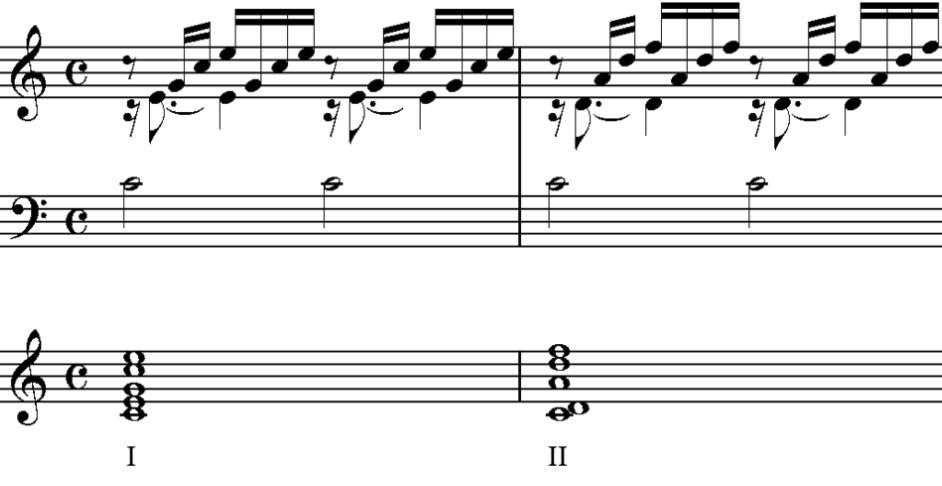
\includegraphics[\linewidth]{eg.png}
  \caption{Two levels of hierarchies in Bach's Preludium in C major \cite{wiki:bach}: the original piece and the underlying chords.
          The details in the first two staffs can be summarised into the chords in the third staff}
  \label{fig:egbach}
\end{figure}

\begin{figure}
  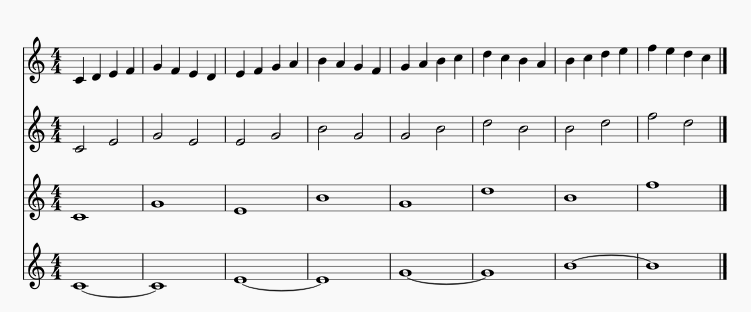
\includegraphics[\linewidth]{egscale.png}
  \caption{Four levels of hierarchies in an artificial example using scales: from the top to the bottom staff, we have different levels of details in different levels of hierarchies.
    The notes at different levels of hierarchies are specified based on the metrical positions of the notes.}
  \label{fig:egscale}
\end{figure}

\textbf{Contributions}
\begin{itemize}
\item  Based on fractal geometry and the hierarchical structures in music, we propose a new feature for symbolic music data.
\item  Using the proposed feature, we present a library for musical analysis and pattern discovery.
\item  We show the effectiveness of our system for musical pattern discovery and compare the proposed feature with other symbolic music features. 
\end{itemize}


\message{ !name(ISMIR2019template.tex) !offset(73) }

\end{document}
